%%%%%%%%%%%%%%%%%%%%%%%%%%%%%%%%%%%%%%%%%%%%%%%%%%%%%%%%%%%%%%%%%%%%%%%%%%
\chapter{Optimalizace velikosti bajtkódu}\label{Tool}

% TODO 
% *
V této kapitole analyzuji obsah vybraného vzorku \texttt{class} souborů a na základě zjištěných poznatků navrhuji metody pro optimalizaci jejich velikosti. 

%%%%%%%%%%%%%%%%%%%%%%%%%%%%%%%%%%%%%%%%%%%%%%%%%%%%%%%%%%%%%%%%%%%%%%%%%%
\section{Analýza bajtkódu}\label{Analysis}

% Popis způsobu analýzy rozsáhlého vzorku testovacích dat, prezentace výsledků a zhodnocení.

Pomocí nástroje \texttt{jbyco} jsem získala data reprezentující vybraný vzorek testovacích souborů a tato data následně zpracovala a vyhodnotila. Zkoumala jsem velikosti položek v~\texttt{class} souborech, užití lokálních proměnných a parametrů metod a typické sekvence instrukcí. Testovací vzorek jsem vytvořila z~\texttt{jar} souborů stažených z~\texttt{http://mvnrepository.com}. Z~populárních kategorií jsem vybrala nejčastěji stahované soubory. Zvolený vzorek se skládal z 95 souborů o celkové velikosti 102,4 MB a obsahoval 59 230 \texttt{class} souborů.

\subsubsection{Velikost položek v souboru}

Typický \texttt{class} soubor z velkého vzorku obsahuje v průměru 117 konstant v tabulce konstant, 2 členské proměnné, 8 metod, 163 instrukcí a 29 atributů. Ze zkoumání celkové velikosti těchto položek vyplynulo, že konstanty tvoří 64\% z celkové velikosti všech souborů, členské proměnné 1\%, metody 2\% a instrukce 10\%.
%Součet velikostí všech atributů ku celkové velikosti souborů tvoří 47\%, ale tato hodnota je nic nevypovídající, neboť atributy mohou být součástí jiných atributů a jejich velikost je tedy započítána vícekrát. 
Nejvýznamnější atributy jsou pak \texttt{Code} s velikostí 30\%, informativní atributy s velikostí 14\% a \texttt{StackMapTable} s velikostí 2\%.

Při bližším pohledu na velikosti konstant se ukázalo, že 89\% z celkové velikosti konstant je tvořen pouze konstantami typu \textit{constant\_utf8}. Tedy konstantami popisujícími řetězce v souboru. Z těchto řetězců pak 61\% obsahuje názvy tříd, metod a členských proměnných a popisy jejich typů. Konstanty popisující číselné a řetězcové hodnoty tvoří 1\% z celkové velikosti konstant a zbývající konstanty pro popisy tříd, metod a proměnných tvoří 10\%.

Zkoumání instrukcí z hlediska jejich velikosti ukázalo, že prvních pět nejobjemnějších instrukcí tvoří 40\% z celkové velikosti instrukcí. Jsou to instrukce pro volání metod, načtení hodnoty z členské proměnné a načtení reference na objekt z lokální proměnné s indexem 0. Na této pozici se často vyskytuje reference na aktuální objekt. Z instrukcí s proměnnou délkou má instrukce \texttt{tableswitch} v průměru velikost 107 B a instrukce \texttt{lookupswitch} velikost 43 B.

% TODO tabulka celkových velikostí
% TODO tabulka řetězců
% TODO tabulka informativních atributů
% TODO tabulka nejčastějších instrukcí

\subsubsection{Užití lokálních proměnných a parametrů metody}

Data popisující užití parametrů a lokálních proměnných jsou znázorněna v grafech \ref{params} a \ref{vars}. Z dat vyplývá, že z lokálních proměnných obsahujících argumenty metody se tyto hodnoty načtou průměrně jedenkrát a dále se s nimi nepracuje. S nižším indexem proměnné počet načítání roste až k hodnotě 2,5 pro index 0. V tomto indexu se u nestatických metod předává reference na aktuální objekt (\texttt{this}). S lokálními proměnnými, které neslouží k předávání parametrů, se průměrně provádí 4,2 operací načítání, 1,8 operací vkládání a 0,3 operací inkrementace.

\begin{figure}[h!]
\centering
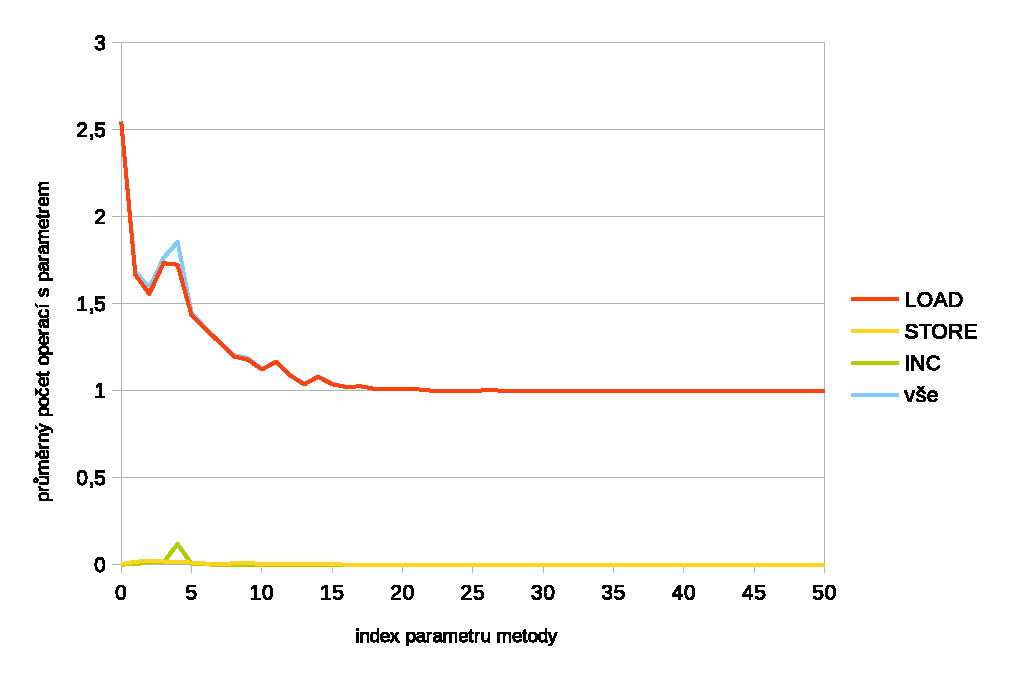
\includegraphics[scale=0.9]{fig/params}
\caption{Průměrné počty operací s parametry metod.}\label{params}
\end{figure}

\begin{figure}[h!]
\centering
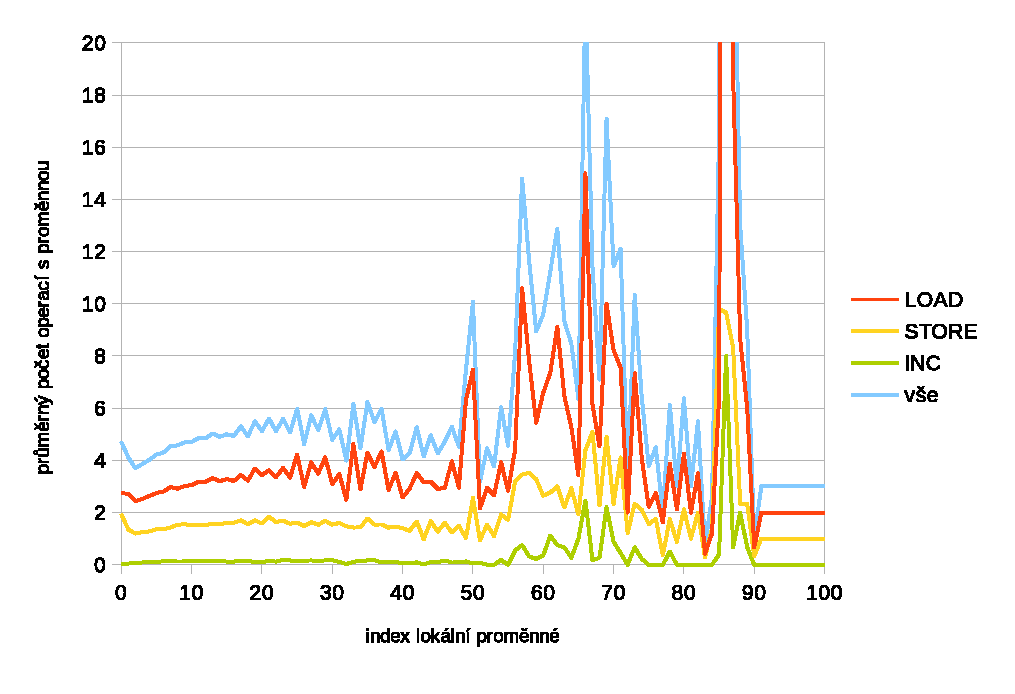
\includegraphics[scale=0.9]{fig/locals} 
\caption{Průměrné počty operací s lokálními proměnnými.}\label{vars}
\end{figure}

% TODO vzory
\subsubsection{Typické operace}

Z dat pro sekvence instrukcí délky jedna vyplývá, že 15,80\% instrukcí tvoří instrukce pro volání metod objektu. Dalšími významnými instrukcemi jsou instrukce pro načtení hodnot z proměnných: čtení z parametru metody 10,41\%, čtení z lokální proměnné 5,64\% a čtení reference na aktuální objekt 9,06\%. Na druhou stranu instrukcí pro ukládání hodnot do proměnných je výrazně méně: uložení do lokální proměnné 2,85\%, uložení do parametru metody 1,40\% a v 49 případech byla hodnota uložena do reference na \texttt{this}. To poukazuje opakované načítání neměnících se hodnot. Obdobně instrukce pro načtení a uložení hodnoty z členské proměnné tvoří 4,53\% a 1,70\%. Pro statické členské proměnné je to 1,16\% a 0,30\%. 

Nejčastěji načítanými typy konstant jsou \texttt{int} 5,91\%, řetězec 2,46\%, reference na \texttt{null} 0,61\%, \texttt{double} 0,24\% a \texttt{long} 0,24\%. Nejčastější instrukcí skoku je nepodmíněný skok 1,77\%. Následují skoky s testy na rovnost 1,22\%, \texttt{null} 0,53\% a nerovnost 0,50\%. Z hlediska práce se zásobníkem jsou zajímavé instrukce pro duplikaci a odebrání vrcholu, které tvoří 3,53\% a 0,88\%. Pro práci s polem pak instrukce pro uložení hodnoty 1,69\%, načtení hodnoty 0,62\% a zjištění délky pole 0,27\%. Ukládání hodnot do pole je tedy častější operací než čtení hodnot z pole. U proměnných to bylo naopak. Kromě instrukce pro vytvoření nového objektu 1,96\% je četnost každé další instrukce pod 1\%. 

Za zmínku dále stojí instrukce \texttt{swap} s 2 315 výskyty, \texttt{nop} s 364 výskyty a instrukce \texttt{lookupswitch} a \texttt{tableswitch}. Ve 21 případech instrukce \texttt{lookupswitch} obsahovala jen adresu výchozího bloku instrukcí, v 552 případech obsahovala jednu dvojici hodnota-adresa a v 998 případech dvě dvojice, což je nejčastější podoba této instrukce. V instrukci \texttt{tableswitch} se nejčastěji pracuje s rozsahem hodnot o délce tři a to ve 442 případech. Ve 150 případech je délka rozsahu 1.

\subsubsection{Typické parametry}

Ze zkoumání konkrétních parametrů instrukcí vyplývá, že nejčastějšími konstantními hodnotami typu \texttt{int} jsou 0, 1, 2, 3, 4, -1, 8, 5, 10, 7, 16 a 255. Typickou konstantou typů \texttt{long} a \texttt{double} je 0 a typickou řetězcovou konstantou je prázdný řetězec. Nejčastější třídou, se kterou se v instrukcích pracuje, je \texttt{java.lang.StringBuilder}. Další typické třídy jsou \texttt{java.lang.Object} a \texttt{java.util.Iterator}.

\subsubsection{Typická těla metod}
% begin - end

\subsubsection{Podmíněné a nepodmíněné skoky}
% neobsahuje skoky, které lze rozhodnout z parametrů - většinou
% LOAD VAR(0); LOAD VAR(0); IFEQ LABEL(0);
% GOTO LABEL(0); GOTO LABEL(1);
% switch
% GOTO LABEL(0); LABEL(0); 
% IFNULL LABEL(0); GOTO LABEL(1);
%IFNE LABEL(0); GOTO LABEL(1);
% LABEL(0); RETURN;
% LABEL(0); GOTO LABEL(1);


\subsubsection{Číselné konstanty a operace nad nimi}
% nahrazení LDC
% ze sčítání na inc
% CONST I(0); SHR;
% CONST I(0); ADD;

\subsubsection{Práce se zásobníkem}
% *, pop, *, return, nop, dup
% duplikace stejných hodnot pomocí dup
% LOAD VAR; NEW OBJECT; DUP_X1; SWAP;
% POP2; RETURN;
% LOAD VAR; LOAD this; SWAP;
% PUTSTATIC OBJECT(0) FIELD(0); GETSTATIC OBJECT(0) FIELD(0); 
% STORE VAR(0); LOAD VAR(0); POP; 
% STORE VAR(0); LOAD VAR(0); RETURN; 
% STORE VAR(0); LOAD VAR(0); 

\subsubsection{Práce s řetězci}
% konkatenace dvou řetězcových konstant před append
% pr8zdný řetězec
% Volání bezparametrické metody.
% String builder, append


\subsubsection{Práce s objekty}
% CONST null; CHECKCAST ARRAY;
% CHECKCAST OBJECT(0); CHECKCAST OBJECT(0); 
% CONST null; ATHROW;

%%%%%%%%%%%%%%%%%%%%%%%%%%%%%%%%%%%%%%%%%%%%%%%%%%%%%%%%%%%%%%%%%%%%%%%%%%
\section{Metody pro optimalizaci velikosti bajtkódu}\label{Analysis}

Výsledky analýzy \texttt{class} souborů jsem uplatnila při návrhu metod pro optimalizaci jejich velikosti. Inspirovala jsem se optimalizacemi, které navrhl Vašek \cite{TODO} nebo které popisuje Aho \cite{TODO}.

\subsubsection{Odstranění zbytečných atributů}
V kapitole \ref{TODO} jsou mezi informativní atributy zařazeny ty, které poskytují informace vhodné například pro ladění programů. Jsou to atributy \texttt{SourceFile}, \texttt{SourceDebugExtension}, \texttt{LineNumberTable}, \texttt{LocalVariableTable}, \texttt{LocalVariableTypeTable} a \texttt{Deprecated}.  Z analýzy vyplynulo, že informativní atributy tvoří 14\% z celkové velikosti zpracovaných \texttt{class} souborů. Vzhledem k tomu, že atributy nejsou důležité pro správnou interpretaci souboru, je žádoucí je ze souboru odstranit.

\subsubsection{Přejmenování balíčků, tříd, metod a členských proměnných}
Více než polovinu z celkové velikosti souborů tvoří řetězce. Mezi tyto řetězce patří mimo jiné řetězcové konstanty, názvy atributů, tříd, metod, proměnných a popisy typů. Součástí popisu typu pak mohou být opět názvy tříd. Jako vhodnou optimalizací se v této oblasti proto nabízí přejmenování balíčků, tříd, metod a členských proměnných za použití co nejkratších názvů. Taková optimalizace ale představuje velký zásah do struktury programu, který nemusí být vždy žádoucí. Je třeba zvážit dva případy. Pokud program slouží jako knihovna, ze které lze importovat balíčky a třídy, pak je třeba zachovat všechny veřejně dostupné názvy. Pokud je program konečnou aplikací zabalenou do \texttt{jar} souboru, pak je možné přejmenovat všechny entity včetně názvu třídy u položky \texttt{Main-Class} v manifestu \texttt{jar} souboru.

% ZMĚNA OD 9.5.2016

\subsubsection{Realokace lokálních proměnných}
Analýza užití lokálních proměnných a parametrů metod odhalila, že se s tímto paměťovým prostorem nepracuje optimálně. K úspornějšímu užívání proměnných nabádá i specifikace \cite{Lindholm:JVM}. Proměnné lze realokovat a recyklovat tak, aby se častěji pracovalo s nižšími indexy proměnných. Nižší indexy pak umožňují používat kratší varianty instrukcí pro práci s proměnnými. Nejvíce užívanými indexy by proto měly být hodnoty 0 až 3, pro které existují specializované jednobajtové instrukce \texttt{load} a \texttt{store}. 

\subsubsection{Vkládání metod}
Pokud je volání metody z hlediska velikosti dražší než provedení těla metody, pak je vhodné toto volání nahradit instrukcemi z těla metody. Pokud se následně tato metoda nikde nevolá, je žádoucí její definici z příslušného \texttt{class} souboru zcela odstranit. Tato optimalizace opět zasahuje do struktury programu jako v případě přejmenování balíčků, tříd, metod a členských proměnných.

%=========================================================================
\subsubsection{Optimalizace práce se zásobníkem}

\begin{tpatterns}

  \code{nop;}
& \code{-}
& \desc{Instrukce \texttt{nop} nemá žádný efekt. Lze ji proto odstranit.} \\

  \code{iconst\_0; \\ pop;}
& \code{-}
& \desc{Pokud instrukce před \texttt{pop} vkládá na zásobník hodnotu o délce jedné jednotky hloubky zásobníku a nemá žádný vedlejší efekt, lze obě instrukce odstranit. Obdobně pro \texttt{pop2.}} \\

  \code{iconst\_0; \\ iconst\_1; \\ swap;}
& \code{iconst\_1; \\ iconst\_0;}
& \desc{Pokud obě instrukce před \texttt{swap} vkládají na zásobník hodnoty o délce jedné jednotky hloubky zásobníku a nemají žádný vedlejší efekt, lze je prohodit a instrukci \texttt{swap} odebrat.} \\

  \code{swap; \\ return;}
& \code{return;}
& \desc{Pokud instrukce před \texttt{return} manipuluje se zásobníkem nebo lokálními proměnnými a nemá žádný vedlejší efekt, lze ji odstranit.} \\

  \code{iconst\_0; \\ new $c$; \\ dup\_x1; \\ swap;}
& \code{new $c$; \\ dup; \\ iconst\_0;}
& \desc{Aplikace instrukcí \texttt{swap} a \texttt{dup\_x1}.} \\

\end{tpatterns}

%=========================================================================
\subsubsection{Duplikace hodnot na zásobníku}

\begin{tpatterns}

  \code{bipush $x$; \\ bipush $x$;}
& \code{bipush $x$; \\ dup;}
& \desc{Pro duplikaci konstantních hodnot lze použít speciální instrukci \texttt{dup}.} \\

  \code{iload $x$; \\ iload $x$;}
& \code{iload $x$; \\ dup;}
& \desc{Dvojí načtení hodnoty z téže lokální proměnné lze nahradit duplikací hodnoty.} \\

  \code{istore $x$; \\ iload $x$;}
& \code{dup; \\ istore $x$;}
& \desc{Místo uložení hodnoty do lokální proměnné a opětovné načtení hodnoty z téže proměnné lze hodnotu na zásobníku duplikovat a kopii uložit do proměnné.} \\

\end{tpatterns}

%=========================================================================
\subsubsection{Substituce číselných konstant}

Číselné konstanty lze vkládat na zásobník více způsoby. Pro některé hodnoty existují krátké specializované instrukce, zatímco jiné hodnoty je nutné vyjádřit pomocí položky v tabulce konstant. Je tedy žádoucí každou instrukci pro vložení číselné konstanty nahradit co nejkratší alternativou. Například tříbajtovou instrukci \texttt{sipush 0} lze nahradit jednobajtovou instrukcí \texttt{iconst\_0}, jak je uvedeno v tabulce \ref{tab:substitution}.

Jednotlivé číselné datové typy jsou v instrukční sadě různě podporované. Například pro hodnotu 3 typu \texttt{int} existuje specializovaná jednobajtová instrukce \texttt{iconst\_3}, ale pro hodnotu 3,0 typu \texttt{double} je třeba použít tříbajtovou instrukci \texttt{ldc2\_w} a devítibajtovou položku v tabulce symbolů. Někdy proto může být vhodnější použít kratší instrukci s jiným typem a výsledek přetypovat, jak ukazuje tabulka \ref{tab:substitution}. Tuto metodu nelze aplikovat současně s metodou zjednodušení algebraických výrazů, neboť by se zápis instrukcí opět zjednodušil. Je ji proto vhodné aplikovat jako poslední krok optimalizace.

\begin{table}[ht]
\begin{tpatterns}

  \code{sipush 0;}
& \code{iconst\_0;}
& \desc{Instrukce pro vkládání číselných proměnných lze někdy nahradit kratšími instrukcemi.} \\

  \code{ldc2\_w 3.0;}
& \code{iconst\_3; \\ i2d;}
& \desc{Drahé instrukce pro vkládání číselným konstant lze nahradit kratšími instrukcemi pro jiný typ a přetypováním.} \\

  \code{ldc2\_w NaN;}
& \code{dconst\_0; \\ dup2; \\ ddiv;}
& \desc{Instrukci pro vložení konstanty \texttt{NaN} lze nahradit instrukcemi pro dělení nulou s plovoucí řádovou čárkou. Ušetří se tak jedna položka v tabulce konstant.} \\

\end{tpatterns}

\caption{Příklady substitucí číselných konstant.}
\label{tab:substitution}
\end{table}

%=========================================================================
\subsubsection{Zjednodušení algebraických výrazů}

% TODO přetypování?

Některé sekvence instrukcí popisující výpočet algebraických výrazů lze zjednodušit nebo zcela nahradit hodnotou daného výrazu. Tato zjednodušení vychází z vlastností matematických operací a specifikace instrukcí. Příklady této optimalizace jsou uvedené v tabulce  \ref{tab:algebra}.

\begin{table}[ht]
\begin{tpatterns}

  \code{iinc $i$ 0;}
& \code{-}
& \desc{Inkrementace lokální proměnné $i$ o nulu nemá žádný efekt.} \\

  \code{iconst\_0; \\ iadd;}
& \code{-}
& \desc{Přičtení nuly nemá žádný efekt. Instrukce lze proto smazat. Obdobně pro \texttt{ishr}, \texttt{ishl}, \texttt{iushr} a instrukce pro typ \texttt{long}.} \\

  \code{ldc NaN; \\ fadd;}
& \code{pop; \\ ldc NaN;}
& \desc{Výsledkem součtu s hodnotou \texttt{NaN} je \texttt{NaN}. Obdobně pro typ \texttt{double}.} \\

  \code{ldc $x$; \\ ldc $y$; \\ iadd;}
& \code{ldc $x+y$;}
& \desc{Jsou-li operandy matematické operace číselné konstanty, pak lze určit výsledek operace. Instrukce je pak možné nahradit tímto výsledkem.} \\

  \code{iload $x$; \\ bipush $i$; \\ iadd; \\ istore $x$;}
& \code{iinc $x$ $i$;}
& \desc{Užití specializované instrukce \texttt{iinc}.} \\

\end{tpatterns}
\caption{Příklady zjednodušení algebraických výrazů.}
\label{tab:algebra}
\end{table}

%=========================================================================
\subsubsection{Optimalizace skoků}

V rámci kódu každé metody lze upravit některé instrukce tak, 

\begin{tpatterns}

  \code{goto $l$;\\ $l$: \dots}
& \code{$l$: \dots}
& \desc{Nepodmíněný skok na bezprostředně následující instrukci lze odstranit, neboť je takový skok zbytečný.} \\

  \code{goto $l_0$; \\ iconst\_0 \\ $l_1$: \dots}
& \code{goto $l_0$; \\ $l_1$: \dots}
& \desc{Pokud instrukce bezprostředně následující za \texttt{goto} není cílem skoku z nějaké instrukce, případně počátkem bloku pro zpracování výjimky, pak ji lze odstranit, neboť se nikdy neprovede. Totéž platí pro instrukce pro návrat z metody.} \\

  \code{goto $l$; \\ \dots \\ $l$:return;}
& \code{return; \\ \dots \\ $l$:return;}
& \desc{Nepodmíněný skok na instrukci pro návrat z metody lze nahradit instrukcí pro návrat z metody.} \\

  \code{goto $l_0$; \\ \dots \\ $l_0$: goto $l_1$;}
& \code{goto $l_1$; \\ \dots \\ $l_0$: goto $l_1$;}
& \desc{Skok na instrukci skoku lze nahradit přímým skokem na cílovou instrukci.} \\

\end{tpatterns}

%=========================================================================
\subsubsection{Optimalizace větvení}

\begin{tpatterns}

  \code{lookupswitch $l$;}
& \code{goto $l$;}
& \desc{Pokud je tabulka dvojic v instrukci \texttt{lookupswitch} prázdná, pak lze tuto instrukci nahradit skokem na výchozí adresu. } \\

  \code{dup; \\ if\_icmpeq $l$;}
& \code{pop; \\ goto $l$;}
& \desc{Duplikovaná číselná hodnota je rovna své kopii. Výsledkem porovnání je proto pravda. Obdobně pro \texttt{if\_icmple} a \texttt{if\_icmpge}.} \\

  \code{dup; \\ if\_icmpne $l$;}
& \code{pop;}
& \desc{Duplikovaná číselná hodnota je rovna své kopii. Výsledkem porovnání je proto nepravda. Obdobně pro \texttt{if\_icmplt} a \texttt{if\_icmpgt}.} \\

  \code{if\_icmpeq $l$; \\ goto $l$;}
& \code{pop2; \\ goto $l$; }
& \desc{V případě rovnosti i nerovnosti hodnot se skáče na stejnou adresu. Porovnávání hodnot je proto zbytečné.} \\

  \code{aconst\_null; \\ ifnull $l$;}
& \code{goto $l$;}
& \desc{Pro referenci na \texttt{null} je výsledkem porovnání s \texttt{null} vždy pravda. Obdobně pro \texttt{ifnonnull}.} \\


\end{tpatterns}

%=========================================================================
\subsubsection{Optimalizace konkatenace řetězců}

\begin{tpatterns}
\end{tpatterns}

%=========================================================================
\subsubsection{Optimalizace práce s objekty}

\begin{tpatterns}
\end{tpatterns}

%=========================================================================
\subsubsection{Optimalizace bajtkódu}

%%%%%%%%%%%%%%%%%%%%%%%%%%%%%%%%%%%%%%%%%%%%%%%%%%%%%%%%%%%%%%%%%%%%%%%%%%
